% id: 102-14
% book: 100발100중 3-1 기말 · 01 3-1 기말(이차방정식·이차함수·부록)
% section: 실전문제 2회 · 02 이차함수 $y=ax^2+bx+c$의 그래프
% figure: crop:fig-102-14.png
% answer: ⑤
% answer_source: 답지(빠른정답)
% variant_level: 0 (원본 전사)
% 이 파일은 build.mjs 가 items.json 에서 만든다. 고칠 때는 items.json 을 고친다.
\smash{\raisebox{1.5mm}{\dmkichul{100발100중 3-1 기말 102쪽 14번}}}
\noindent\begin{minipage}[t]{0.58\linewidth}\vspace{0pt}\raggedright 이차함수 $y=ax^2+bx+c$의 그래프가 그림과 같을 때, $-a+b+c$의 값은? \cond{$a$, $b$, $c$는 상수이다.}\end{minipage}\hfill\begin{minipage}[t]{0.4\linewidth}\vspace{0pt}\centering 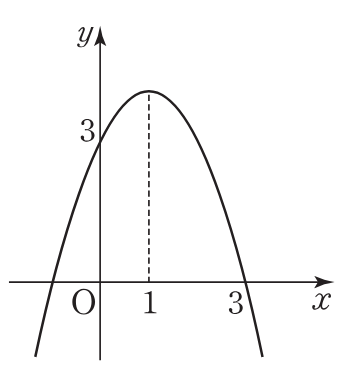
\includegraphics[width=82.2pt]{figures/fig-102-14.png}\end{minipage}\par
\begin{choicesii}{$2$}{$3$}{$4$}{$5$}{$6$}\end{choicesii}
